\documentclass[]{article}
\usepackage{lmodern}
\usepackage{amssymb,amsmath}
\usepackage{graphicx}
\usepackage{ifxetex,ifluatex}
\usepackage{fixltx2e} % provides \textsubscript
\usepackage[T1]{fontenc}
\usepackage[utf8]{inputenc}

\usepackage[verbose,tmargin=2cm,bmargin=2cm,lmargin=2.5cm,rmargin=2.5cm]{geometry}

\usepackage{color}
\definecolor{grey}{rgb}{0.5, 0.5, 0.5}

\usepackage[unicode=true]{hyperref}
\urlstyle{same}  % don't use monospace font for urls
\hypersetup{breaklinks=true,
            bookmarks=true,
            pdfauthor={Daniel Falster, Rich FitzJohn, Mark Westoby},
            pdftitle={TREE: A package for modelling plant TRait Ecology and Evolution},
            colorlinks=true,
            citecolor=grey,
            urlcolor=grey,
            linkcolor=grey,
            pdfborder={0 0 0}}

\usepackage{lineno}
\linespread{2}

\usepackage[colorinlistoftodos]{todonotes}

\usepackage{authblk}
\title{TREE: A package for modelling plant TRait Ecology}
\author[1]{Daniel S. Falster}
\author[1]{Richard G. FitzJohn}
\author[1]{Mark Westoby}
\affil[1]{Dept of Biological Sciences, Macquarie University, Sydney, NSW 2109, Australia}
\date{}

\usepackage{natbib}
\bibliographystyle{mee}

\usepackage[title,titletoc,toc]{appendix}

\begin{document}
\maketitle

A manuscript in consideration as a research paper for publication in MEE
as part of the Special Feature Demography beyond the Population

\listoftodos

\linenumbers

\section{Abstract}\label{abstract}

\emph{(max 350 words; rework into 4 points)}

\begin{enumerate}
\def\labelenumi{\arabic{enumi}.}
\itemsep1pt\parskip0pt\parsep0pt
\item
  Population dynamics in forests are strongly size-structured. Larger
  plants shade smaller plants. They also expend proportionately more
  energy on their woody stems. Although the importance of size-
  structure for demography is widely recognised, many mechanistic models
  either omit it entirely, or include only coarse approximations.
\item
  Here we introduce the TREE package (TRait Ecology and Evolution), an
  extensible framework for modelling plant demography across the entire
  life cycle via coupled differential equations. At its core, TREE is an
  individual-based mechanistic model where plant function is mediated by
  traits, Individuals from multiple species can be grown in isolation,
  in patches of competing plants, or in metapopulations under a
  disturbance regime. Dynamics within patches of competing plants are
  resolved using novel extensions of the Escalator Boxcar Train
  technique. Combined effects of trait-, size- and patch-structured
  dynamics are integrated into population level estimates of
  reproductive fitness.
\item
  TREE is presented as an open source \texttt{R} package and is
  available at
  \href{https://github.com/traitecoevo/tree}{github.com/traitecoevo/tree}.
  While accessed from R, the core routines in TREE are written in C++.
  The package provides for alternative physiologies and for
  hyper-parameterisation on the basis of plant functional traits. A
  detailed test suite is provided to ensure accuracy.
\item
  We provide worked examples illustrating TREE's use to study the
  influence of functional traits on growth of individual plants, of
  whole stands and on assembly of ecological communities.
\end{enumerate}

\textbf{Key-words}: demography, emergent property, fitness, growth,
physiology, metapopulation, mortality, reproduction, size-structure,
trade-off

\section{Introduction}\label{introduction}

Plant growth and demography are fundamentally structured by species
traits and by individual size. Both influence dynamics over time-scales
ranging from instantaneous physiological effects to long-term
evolutionary outcomes \citep{Harper-1977, Westoby-2002}. As an
individual increases its leaf area, its potential to generate
photosynthate also rises. But for larger individuals, increasing
fractions of photosynthetic income must also be diverted towards
building and maintaining support tissues rather than leaves
\citep{Givnish-1988, Enquist-1999}. A larger fraction of income is also
allocated to reproduction \citep{Thomas-2011}. Consequently at
population level, rates of growth and mortality change with size
\citep{Muller-2006, Thomas-2011, Ruger-2011, Wright-2010}. The traits of
a species also interact with size to shape its demography. Leaf
construction costs and wood density affect growth rates
\citep{Wright-2010}. Other traits such as seed size and height at
maturation determine start and end points of ontogenetic trajectories
\citep{Westoby-2002}. Over longer time-frames, natural selection favours
traits making plants more competitive such as faster growth, larger
seeds, taller height \citep{Falster-2003}. Selective forces thus
potentially amplify size-related effects on demography. Accounting for
the effects of size and traits in models therefore seems like a key step
in developing theory for the structure and dynamics of the biosphere
\citep{Purves-2008, Moorcroft-2001, Falster-2003}, in particular notable
phenomena such as successional dynamics, self thinning, trait evolution
and species coexistence.

Although the importance of size-structure for vegetation function and
demography has been widely recognised for a long time
\citep{Harper-1977, Hara-1984, Shugart-1980, Huston-1987, Moorcroft-2001, Kohyama-1993, Enquist-1999, Pacala-1996, Coomes-2007},
most large-scale mechanistic models of plant growth either omit it
entirely, or include only coarse approximations
\citep{Cramer-2001, Sitch-2003}. The likely reason is the computational
challenge of modelling size-structured dynamics. During the 1980s and
early 1990s, size-structured ``gap'' models were widely used
\citep[e.g.][]{Huston-1987, Shugart-1980}. These gap models were
parameterised in terms of growth and demography, and consequently did a
poor job of simulating carbon fluxes. The next generation of models
focussed more on physiology and, presumably for computational reasons,
sacrificed details of demography in order to achieve global coverage
\citep[eg.][]{Haxeltine-1996}. This history has brought us to the
current perplexing situation where all but a couple
\citep[e.g.][]{Moorcroft-2001, Smith-2014} of the leading vegetation
models lack size-structure
\citep{Cramer-2001, Dekauwe-2014, Sitch-2003, Kelley-2013}. These models
are focused on modelling fluxes carbon and water, but say little about
demographic behaviour, and consequently are also unable to account for
any non-linear demographic feedbacks that may arise.

Interestingly, most models used in theoretical ecology to explore
questions about species coexistence also lack size-structured dynamics
\citep[e.g.][]{MacArthur-1967, Levin-1974, Leimar-2013, Geritz-1995, Calcagno-2006, Tilman-1985}.
It is common to assume competitive interactions are influenced by
size-related traits such as adult and seed size, but detailed
size-structured demography is rarely considered, at least for plant
models \citetext{\citealp[for animal
examples,][]{Deroos-1988}; \citealp[see][]{Deroos-1992}}. Thus it has
been difficult to connect mechanisms described in these simplistic
models with field data and real traits, which are almost always strongly
size-structured.

In this note, we describe the \texttt{TREE} package for R
\citep{R-2015}, a mechanistic framework for studying the effects of size
structure and trait variation on the demography of individual plants, of
patches of competing plants, and of meta-populations structured by a
prevailing disturbance regime. The package came about as a way to extend
previous work investigating the effect of traits on vegetation
properties \citep{Falster-2011} and the mechanisms facilitating
coexistence of trait mixtures \citep{Falster-2015}. These studies
provided the foundation methods needed; here we provide robust and
extensible implementations. We describe the general approach of the
package and then a series of use cases, focussing at different levels of
ecological organisation. Each section provides a short description of
the required methods, design considerations, and then some worked
examples illustrating potential use cases and design features. Detailed
technical documents are provided as supplementary information, and updated
versions of technical documents are also available within the TREE
package itself. The use cases highlighted reflect our own interests in
understanding trait-based demography and community assembly. Yet we
expect the methods provided to be useful in other contexts. For example,
prior to TREE there was no R package that allowed one to simply grow a
plant over time, based on well-understood physiology. Surely this is one
of the simplest demographic actions one might hope for, with diverse
potential applications in ecology, evolution, forestry, agriculture, and
vegetation modelling. We hope the mechanistic platform provided here
will complement the increasingly sophisticated statistical methods now
available to analyse size-structured data \citep[e.g.][]{Metcalf-2013}.

\section{The methods}\label{the-methods}

TREE is a mechanistic model, meaning the dynamics of the system arise
from rules specifying on how individuals grow and interact. In ecology,
there is a long history of using simple deterministic models \citep[such
as Lotka-Volterra population dynamics,
e.g.][]{MacArthur-1967, Leimar-2013} to understand biological phenomena.
TREE was developed with this style of analysis in mind, while also
allowing for a richer set of ecological dynamics than is possible in
population models lacking size structure. The package implements methods
for physiological, population, and adaptive dynamics (Fig.
\ref{fig:schematic}) following methods described by \citet{Falster-2011}
and \citet{Falster-2015}. The core rules in TREE are about the
short-term physiological functioning of an individual plant and how
these are influenced by its traits, size and light environment. Dynamics
at higher levels of organisation then arise as emergent properties,
driven by growth physiology, competition for light and disturbance (Fig.
\ref{fig:schematic}). Demographic phenomena can be studied at the three
levels of individual plants, stands of competing plants, and entire
metapopulations.

\section{Effects of size, trait and environment on demography of
individual
plants}\label{effects-of-size-trait-and-environment-on-demography-of-individual-plants}

The core of TREE is a model for a plant's physiological strategy as
specified by its traits (Fig. \ref{fig:schematic}a). This sub-model
estimates rate of biomass production for a plant, given its size, light
environment, and the supplied physiological constants. Assimilation is
estimated from total leaf area and the light distribution across the
plant's canopy. Costs of tissue respiration and turnover are then
subtracted. The remaining biomass is then allocated between growth and
reproduction. The strategy model thus includes a list of physiological
rules and associated parameters.

The core job of the physiological model is to take size, light
environment and parameters as inputs, and to return growth rate,
mortality and fecundity as outputs, in other words to move from
individual growth to demography. However additional quantities are also
available as output, such as total assimilation and the respiration,
turnover, and allocation rates for different tissues.

The default physiological model used in TREE largely reflects that
presented in Falster-2011, but with extensions allowing for diameter
growth also to be estimated. To properly model trait variation,
different parameters in the model are linked via assumed trade-offs. For
example, the trait LMA is used to estimate the rate of leaf turnover,
based on widely observed scaling relationship from \citet{Wright-2004}.

\subsection{Design features}\label{design-features}

TREE includes a default physiological model (fully described and derived
in the Appendix \ref{sec:FFW16}). However a feature of the package is that alternative
physiologies can be used, and the parameters of each model can be
altered. Trait differences are accounted for by altering relevant
parameters. This example shows how to establish a new plant with height
of 5 m, and estimate its physiological and demographic rates in the
given light environment.

\begin{verbatim}
# Example illustrating use of individual plant, all the outputs from plant internals
\end{verbatim}

\subsection{Use cases and examples}\label{use-cases-and-examples}

\todo[inline]{these aren't demographic rates - they're
physiological perphaps? Height growth rate, allocation, WPLCP, etc are
properties of individuals here. I've updated but we can discuss.}
\todo[inline]{allocation to replacement costs are not shown in
the figure at all, so this section is quite confused. I've reworded but
you'll want to go through and tweak. The graph shows ``fraction of live
mass that is X'' which is different to what is talked about.}

With above functionality, TREE can be used to estimate essential
physiological rates for individual plants (Fig. \ref{fig:plant}). The
function \texttt{grow\_plant\_to\_size} takes a given strategy and light
environment and grows the plant, producing a trajectory of size over
time (Fig. \ref{fig:plant}a). This is achieved by integrating an
Ordinary Differential Equation (ODE) of size-dependent growth rate (see
Appendix \ref{sec:demography} for more
details). As the plant grows, allocation to different types varies, and
the composition of the plant changes to become more stemmy and less
leafy (Fig. \ref{fig:plant}b). This in turn affects maintenance and
turnover costs and the growth rate of plants (Fig. \ref{fig:plant}c).
This shift alone generates a distinctive hump-shaped pattern of absolute
growth with size, and equally the widely regarded decline in relative
growth rate with size from birth onwards.

By varying the light environment and measuring growth rate, the whole
plant light compensation point (WPLCP) can be computed (Fig.
\ref{fig:plant}d). The WPLCP is increasingly regarded as the most useful
measure of a strategy's shade tolerance
\citep{Givnish-1988, Baltzer-2007, Lusk-2013}. As expected, WPLCP
increases with plant size, due to increased costs of building and
maintaining stem and leaf tissues \citep{Givnish-1988}. Likewise, WPLCP
decreases with LMA, because high LMA species have lower leaf turnover
\citep{Baltzer-2007, Lusk-2013}.

\section{Plants competing in a patch}\label{plants-competing-in-a-patch}

Within patches of competing plants, competition for light generates
strong non-linear feedbacks on growth, survival and reproduction. In the
\texttt{FFW16} physiological model, we consider only the effect of
shading on rates of biomass production, although competition for other
resources such as nitrogen or water could also be considered with
suitable extensions.

Modelling the development of a competitive hierarchy within a patch
requires that both the initial size distribution and the inflow of new
recruits be specified. We have primarily been interested in dynamics of
a patch recovering from disturbance, and have therefore started with an
empty patch and constant flow of seeds from a global seed rain (Fig.
\ref{fig:schematic}b).

\subsection{Design features}\label{design-features-1}

When modelling a patch, we are interested in modelling changes in the
size-density-distribution \(n(h,a)\) over time, i.e.~the density of
individuals with height \(h\) within a patch of age \(a\). We assume
that patches are large, and are vertically but not horizontally
structured. Thus, shading in TREE is modelled as a mean field with
respect to spatial layout. Similar assumptions are found in many models
simulating size-structured dynamics
\citep{Moorcroft-2001, Huston-1987, Smith-2014}. Under these
assumptions, the dynamics of \(n\) behave deterministically and can be
approximated via a Partial Differential Equation (PDE) (see Appendix
\ref{sec:demography}). The same PDE has been shown to capture average behaviour
across a large number of small patches \citep{Moorcroft-2001}. Ideally
one would also consider full spatial interactions within patches,
however such models are very computationally demanding, and also
impossible to solve in a deterministic fashion \citep{Pacala-1996}.
Moreover, it remains unclear whether resolving spatial details within a
patch would provide further ecological detail, in part because the
process of competitive thinning tends to break down spatial clusters
\citep{Strigul-2008}.

Our approach for modelling solving size-structured population dynamics
is based on the Escalator Boxcar Train technique (EBT)
\citep{Deroos-1997, Deroos-1992, Deroos-1988}. The EBT solves the PDE
describing development of \(n\) by approximating the density function
with a collection of cohorts spanning the size spectrum. Following a
disturbance, a series of cohorts are introduced into each patch. These
cohorts are then transported along the characteristic equations of the
PDE. Biologically these are the growth trajectories of individuals,
conditioned on them surviving. Fig. \ref{fig:patch}a illustrates the
trajectories of individuals within a patch recovering from disturbance.
Fig. \ref{fig:patch}b shows the same trajectories, but with shading
indicating the density of plants at that size. (see also Fig.
\ref{fig:schematic}b).

We introduce two extensions to the EBT: i) a new method for estimating
the size-density distribution, and ii) a technique for handling strong
size-asymmetric competitive feedbacks, such as occur under strong
competition for light. The original EBT
\citep{Deroos-1997, Deroos-1992, Deroos-1988} proceeds by approximating
the first and second moments of the density distribution \(n\) within
each cohort. In TREE we use a different but from a theoretical
perspective equally valid approach. Instead of tracking first and second
moments of the size-distribution within cohorts, we track a point mass
estimate of \(n\) along the trajectories corresponding to the boundary
of each cohort. We found this approach preferable because it does not
require us to maintain a separate set of equations for the smallest
cohort \citep{Deroos-1997}.

The extension for handling strong size-asymmetric competition involves
adaptive refining of time points at which new cohorts are introduced
into the population. Under competition, the growth trajectories of
individuals born at similar times can diverge substantially over time
(Fig. \ref{fig:patch}a). This is can become a problem later during patch
development because much of the population can be located between
widely-spaced cohorts, delivering low numerical precision. To maintain
numerical precision we use an iterative algorithm to adaptively refine
the cohort spacing until the trajectories of adjacent cohorts remain
adequately resolved throughout development of the patch (Fig.
\ref{fig:characteristics}b; see Appendix\ref{sec:demography} for details).

\subsection{Use cases and examples}\label{use-cases-and-examples-1}

Modelling of size-structured dynamics via solving of a deterministic PDE
enables multiple complex non-linear demographic phenomena to be
investigated.

Firstly, TREE can simulate patterns of stand development after
disturbance, including self-thinning behaviours and successional
replacement. Whereas previous approaches for modelling self-thinning
were limited to a single species
\citep[e.g.][]{Barnes-2004, Coomes-2007}, TREE accommodates multiple
different species with different traits (Fig. \ref{fig:schematic}b; Fig.
\ref{fig:patch}).

Second, TREE allows for the effects of competition and succession on
productivity and biomass accumulation within a stand to be investigated
\citep{Falster-2011}. Leaf area cover and rates of biomass production
tend to vary with stand age. Such changes might come about via a
combination of physiological and structural changes
\citep{Binkley-2002, Smith-2001, Ogawa-2010, Coomes-2007}. TREE enables
the effects of competitive feedbacks to be incorporated, in addition to
any intrinsic physiological factors. Moreover, TREE allows for the
contributions of different species to be mapped (Fig. \ref{fig:patch}c).

\section{Trait, size and patch structured
vegetation}\label{trait-size-and-patch-structured-vegetation}

Most vegetation is subject to a disturbance regime, such that patches of
the landscape are cleared at some rate, by fire, cyclone, landslide, or
disease outbreak
\citep{Connell-1978, White-1979, Chambers-2013, Bormann-1979, Clark-1991, Coomes-2007}.
The vegetation thus comprises a collection of patches differing in time
since last disturbance and linked via seed dispersal (Fig.
\ref{fig:schematic}a). Such a system is often refereed to as a
structured metapopulation \citep{Gyllenberg-2001}.

\subsection{Design features}\label{design-features-2}

Having simulated a single patch, it is straightforward to scale up from
a single patch to an entire metapopulation, at least for the situation
of metapopulations at an equilibrium mix of patch ages and where
disturbances remove all established vegetation. The frequency-density
\(p(a)\) of patches age \(a\) in the landscape is needed. Assuming there
are a large number of patches means the dynamics of \(p\) behave
deterministically and can be approximated via a second PDE
\citep{Vonfoerster-1959, Mckendrick-1926} (see Appendix
\ref{sec:demography} for
details). Scaling from patch to metapopulation is then achieved by
weighting the temporal dynamics of a single patch by \(p(a)\), the
relative abundance of patches age \(a\) in the metapopulation.

\todo[inline]{This should be largely dealt with now, but vignette
needed.MW: Not clear to me (and the fig doesn't exist yet) --
isn't the seed rain an output property? -- what's it at equilibrium
with? (besides just being stable because the age dist of patches has
stabilized)} The main numerical challenge in stepping from single patch
to metapopulation is to identify the equilibrium seed rain of the
metapopulation. For a given input seed rain, the model produces an
output seed rain. The equilibrium seed rain is the vector of seed rain
where input seed rain equals output seed rain. Finding this equilibrium
requires finding a root of a multidimensional function, subject to the
constraints that this root is stable (e.g., the trivial equilibrium of
zero seed rain always exists, but is often not stable).

\subsection{Use cases and examples}\label{use-cases-and-examples-2}

As previously noted \citep{Kohyama-1993, Moorcroft-2001, Falster-2011} a
feature of the size-structured metapopulation concept implemented here
is that it reconciles equilibrium and non-equilibrium approaches to
modelling ecological dynamics
\citep{Levin-1974, Bormann-1979, Connell-1978, Coomes-2007}. An
equilibrium may be approached at the level of metapopulation, meaning
the seed rain and size structure across the entire metapopulation is
approximately stable. Yet the structure of vegetation within individual
patches is constantly in flux. Patches continue to age and their
residents continue to grow until they are disturbed.

Beyond its conceptual appeal, this idea of a dynamic equilibrium allows
us to close the demographic feedback loop and thereby create a
self-regulating system. The equilibrium seed rain for multi-species
communities is approached demographically, incorporating the combined
effects of the model's physiological rules, species traits, competitive
interactions and the prevailing disturbance regime on the
size-distributions of plants within a metapopulation of patches. Unlike
some vegetation models, there is no need to set the density of seeds or
seedlings, these arise as outputs from the model. Characteristics of the
vegetation such as total leaf area, biomass, productivity and allocation
to different plant parts arise as emergent properties (Fig.
\ref{fig:patch}). Similarly, we can observe emergent patterns for
size-distribution, growth and mortality (Fig. \ref{fig:emergent}).

\section{Invasion fitness}\label{invasion-fitness}

With the extension to metapopulation, we are modelling demography across
the entire life cycle and are thus in a position to estimate the fitness
of different types. Invasion fitness quantifies the ability of a rare
individual with particular traits to establish in a community of
established residents at their equilibrium densities. Invasion fitness
is ideally calculated as the long-term per capita growth rate of the new
type; however, in structured metapopulations, the most convenient
indicator of per-capita growth rate is given by the logarithm of the
basic reproduction ratio \citep{Gyllenberg-2001, Metz-2001}. The basic
reproduction ratio \(R\) is simply the total seed output of the new
type, averaged across the metapopulation. The new type can invade when
\(R > 1\).

\subsection{Use cases and examples}\label{use-cases-and-examples-3}

With fitness defined, it becomes possible to model adaptative dynamics
and community assembly \citep{Dieckmann-2007, Geritz-1998}. This is best
thought of as occurring on a fitness landscape, a surface with fitness
plotted against one or more species traits (Fig \ref{fig:fitness}). The
reproductive success of individuals possessing a particular trait value
is measured in the size- and patch-structured metapopulation, and
depends on both the traits and densities of other species in the current
resident community. The reason this is interesting is that under
frequency- and density-dependence, evolution tends to favour different
trait mixtures compared to those predicted by models that optimise some
feature of the community, such as total biomass or carbon production or
seed production in the absence of competition
\citep{Falster-2003, Dieckmann-2007}.

\todo[inline]{this now comes too close to the caption; reworded
to say something a little broader here.}

Fitness landscapes will be positive in regions that allow invasion, and
zero for species that are at equilibrium. The slope of the fitness
landscape at a resident indicates the direction of selection; a negative
slope (dashed line in Fig. \ref{fig:fitness}a) indicates selection for
smaller trait values. Following the fitness gradient, traits may
encounter evolutionary branching points (\todo[inline]{ dfalster-  please add appropriate adaptive dynamics reference
here}; at this point there is no directional selection (solid line in
figure \ref{fig:fitness}a) but invasion is possible both above and below
it in trait space. The distortions of the fitness landscape as species
are introduce show the strong frequency dependent selection that emerges
from the model through the demographic interactions.

\todo[inline]{dfalster - please finesse/delete that last
line.}

Adding in additional species further ``draws down'' the fitness
landscape. Depending on where additional species are added, the first
species may be selected on, and further invasion may or may not be
possible (Fig. \ref{fig:fitness}b, dotted lines). It is often possible
to find a configuration where fitness is negative everywhere (solid line
in Fig. \ref{fig:fitness}b) except for the zero points where species are
present. This community is immune to invasion from any other strategies.

Identifying conditions promoting trait diversity is a valuable use-case
for TREE. Coexisting plant species differ in a range of physiological
traits, yet the conditions allowing for these different types to coexist
in face of competition for a common set of resources remain largely
unknown. The simple example here can be extended to multiple dimensions
and can be used to investigate how trade-offs facilitate coexistence
\citep{Falster-2015}

\section{Implementation details}\label{implementation-details}

TREE is written in C++ and R, using the package \texttt{Rcpp}
\citep{Eddelbuettel-2011, Eddelbuettel-2013} to bridge between the two
languages. Due to the computationally intensive nature of the model, the
core physiological and demographic components are in C++ to maximise
speed. We used templated types allow the demographic and evolutionary
components to be driven by alternative physiological models while
retaining the same interface at higher levels. Despite mostly being
programmed in C++, all components of the model, down to individual
plants, can be extracted and interacted with dynamically in R, using the
\texttt{RcppR6} package \citep{RcppR6}.

TREE makes use of much existing software, including the programming
language C++; the R computational environment \citep{R-2015}, the R
packages \texttt{Rcpp} \citep{Eddelbuettel-2011, Eddelbuettel-2013},
\texttt{R6}\citep{Chang-2014}, and \texttt{testhat}
\citep{Wickham-2011}; and the Boost Library for C++
\citep{Schaling-2014} via the R package \texttt{BH}
\citep{Eddelbuettel-2015}. Source code is hosted at
\href{https://github.com/traitecoevo/tree}{github.com/traitecoevo/tree}.
Installation instructions are available at this homepage, and binary
releases will also be available there.

\section{Closing comments}\label{closing-comments}

The use-cases described here arise from our interest in the assembly of
trait mixtures in communities. They are nested at different scales
within that question. However a variety of other uses would be possible,
and also extensions to address other facets of community assembly.

Rather than provide a model with a few routines, we have developed an
extensible framework that we hope can be used to answer a number of
questions.

The physiology of growth could be modified, for example to account for
rising atmospheric CO2. - (MW) my suggestion here would be more to
emphasize what you've been saying about using it for growth of
individuals or of stands, rather than the future directions we are
interested in

\begin{itemize}
\item
  Compare to IPM approach
\item
  mathematics similar, difference is source of variability
\end{itemize}

\section{Acknowledgements}\label{acknowledgements}

DS Falster was supported by an ARC discovery grant (DP110102086). RG
FitzJohn was supported by the Science and Industry Endowment Fund
(RP04-174). M Westoby was supported by a fellowship from Australian
Research Council.

\clearpage
\bibliography{refs.bib}

\clearpage

\section{Figures}\label{figures}

\begin{figure}[h!]
\centering
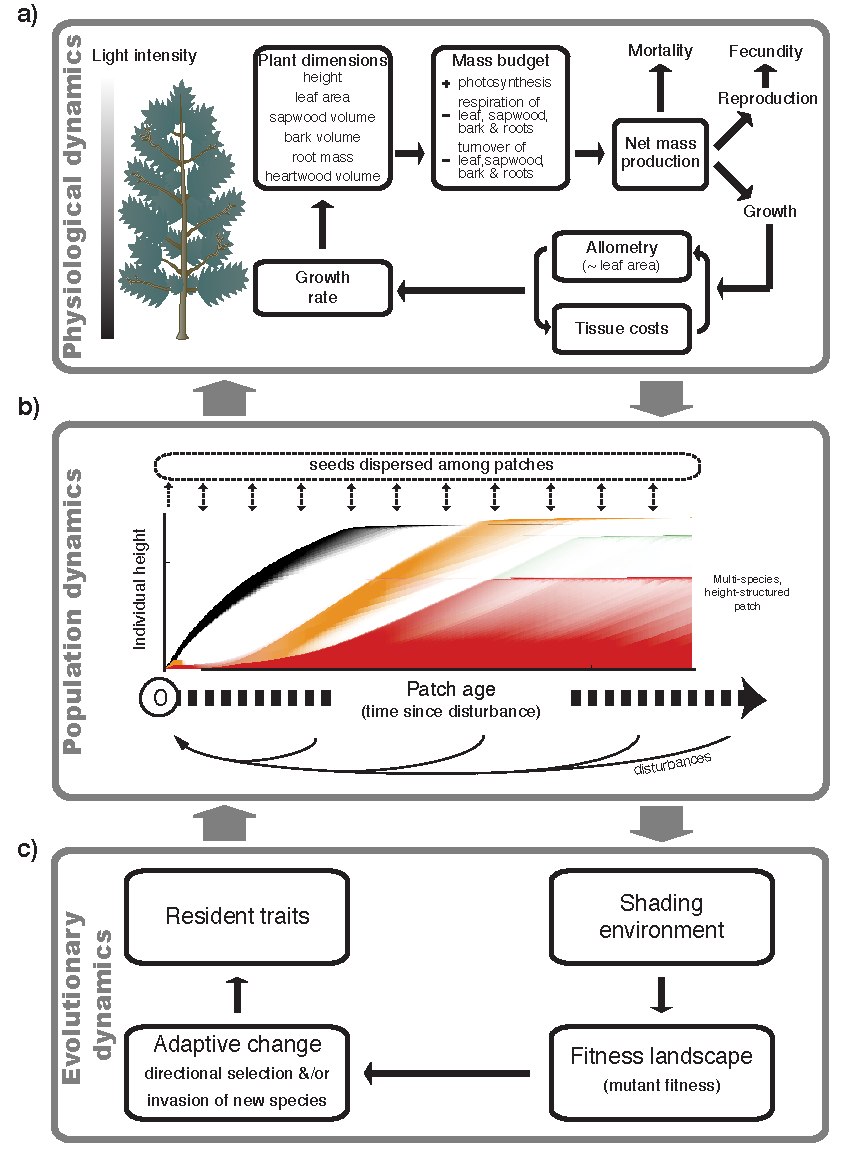
\includegraphics[width=15cm,height=15cm,keepaspectratio]{output/schematic}
\caption{\textbf{Overview of processes included in TREE package,
including physiological dynamics, population dynamics, and evolutionary
dynamics.} \textbf{a,} An individual's vital rates are jointly
determined by its light environment, height, and traits. \textbf{b,} A
metapopulation consists of a distribution of patches linked by seed
dispersal. Disturbances occasionally remove all vegetation within a
patch. Competitive hierarchies within developing patches are modelled by
tracking the height distribution of individuals across multiple species
(distinguished by colours) as patches age after a disturbance. The
intensity of shading indicates the density of individuals at a given
height. \textbf{c,} The traits of the resident species determine the
shading environment across the metapopulation, which in turn determines
fitness landscapes. Resident traits adjust through directional selection
up the fitness landscape and through the introduction of new species
where the fitness landscape is positive. Adapted from Falster *et al.* (2015).
\label{fig:schematic}}
\end{figure}

\newpage

\begin{figure}[h!]
\centering
\includegraphics[width=15cm,height=15cm,keepaspectratio]{output/plant.pdf}
\caption{\textbf{Growth trajectories.} Individual plant height growth with different LMA values and light environments.  (a) Lower light environments flatten growth trajectories, and different species traits have nonlinear interactions with the light level.  (b) Over time, the fraction of living tissue switches from leaf towards sapwood, with high LMA species having relatively more mass in leaf than low LMA species.  (c) Growth rates peak around 5m high, but this position varies with both trait and light level (not that this is the derivative of panel (a)).  (d) Growth rates vary with plant size (seedling and mature shown) and with traits; growth rate differences are more pronounced in low light.  Whole plant light compensation points emerge from the model as the point where growth rate is zero (x intercept).  The light level for panels (a) and (c) is indicated with dots.  Throughout "low LMA" is 0.1 and solid lines, "high LMA" is 0.267 and dashed.
\label{fig:plant}}
\end{figure}

\newpage

\begin{figure}[h!]
\centering
\includegraphics[width=15cm,height=15cm,keepaspectratio]{output/patch.pdf}
\caption{Cohorts of two species growing within a competitive environment.  Each line represents a "cohort"; some number of individuals that share a birth time.  Red lines are the low LMA species from figure \ref{fig:plant}, blue lines are the high LMA species.  The initial growth rate advantage of the low LMA species (see Figure \ref{fig:plant} c) means it quickly overtops the high LMA species, suppressing its growth.  Self-thining leaves space for the high LMA species to invade.  (a) all cohorts, equally weighted; the spacing is generated by an adaptive refinement algorithm.  (b) Cohorts shaded by by their density.  (c) The leaf area index at ground level for each species.  The dotted line is the total leaf area index (sum across both species).}
\label{fig:patch}
\end{figure}

\newpage

\begin{figure}[h!]
\centering
\includegraphics[width=15cm,height=15cm,keepaspectratio]{output/empty.pdf}
\caption{\textbf{Emergent size-distributions across metapopulation}
\label{fig:emergent}}
\end{figure}

\newpage

\begin{figure}[h!]
\centering
\includegraphics[width=15cm,height=15cm,keepaspectratio]{output/fitness.pdf}
\caption{Example fitness landscape for LMA, showing potential for stable coexistence of multiple types.  Fitness is the log of the population growth rate - at zero species are at equilibrium, above zero they will increase in density.  (a) Landscae generated by a single species.  At LMA of 0.1 (the dashed line) there is directional selection for smaller LMA.  At LMA of 0.08 (solid line) there is a branching point (inset).  (b) Landscape generated by two species, holing the first at LMA of 0.08. Introducing a species at the maximum fitness value from panel (a) reduces the region of positive fitness considerably (dashed line).  Dotted lines show subsequent invasions and replacements of the second species, and the solid line shows a stable fitness landscape where both species exist on a peak in the fitness landscape.  At this point no futher invasion is possible.}
\label{fig:fitness}
\end{figure}

\clearpage

\begin{appendices}\label{sec:appendices}
\renewcommand{\thefigure}{S\arabic{figure}}
\renewcommand{\thetable}{S\arabic{table}}

\setcounter{figure}{0}
\setcounter{table}{0}


\section{Default physiological model for TREE}\label{sec:FFW16}

See attached file \url{tree_physiology.pdf}

\section{Modelling demography in the TREE package}\label{sec:demography}

see attached file \url{tree_demography.pdf}


\section{Supplementary figures}\label{supplementary-figures}

\begin{figure}[h!]
\centering
\includegraphics[width=15cm,height=15cm,keepaspectratio]{output/empty.pdf}
\caption{\textbf{Adpative cohort spacing solves problem of diverging characteristics}}
\label{fig:characteristics}
\end{figure}

\newpage

\begin{figure}[h!]
\centering
\includegraphics[width=15cm,height=15cm,keepaspectratio]{output/empty.pdf}
\caption{\textbf{Approach for solving equilibrium seed rain across the metapopulation \todo[inline]{RGF: I favour referring to a package vignette here - I've started rebuilding one that we used to have}}}
\label{fig:seed_rain}
\end{figure}

\end{appendices}
\end{document}
